\section{Validation}
\subsection{Comparison of inbending and outbending data}
One of the validation tests performed on our data is to see if the results are independent of the torus-field polarity.  The first stage of this test is to select only events in the region of overlap between the two configurations.  For the data with the in-bending (out-bending) configuration, particles with positive (negative) charge can be observed at smaller polar angles\footnote{at the interaction point} than in out-bending (in-bending) configuration.  This is demonstrated in Figs.~\ref{fig:p_vs_th_inout_e}, \ref{fig:p_vs_th_inout_h1} and \ref{fig:p_vs_th_inout_h2}, which contain $p$ vs $\theta$ scatter plots of the in-bending (blue) and out-bending (orange) datasets (respectively  for $e$,$h_1$ and $h_2$).  Each of the panels shows a different configuration of hadron types.    

\begin{figure}
    \centering
    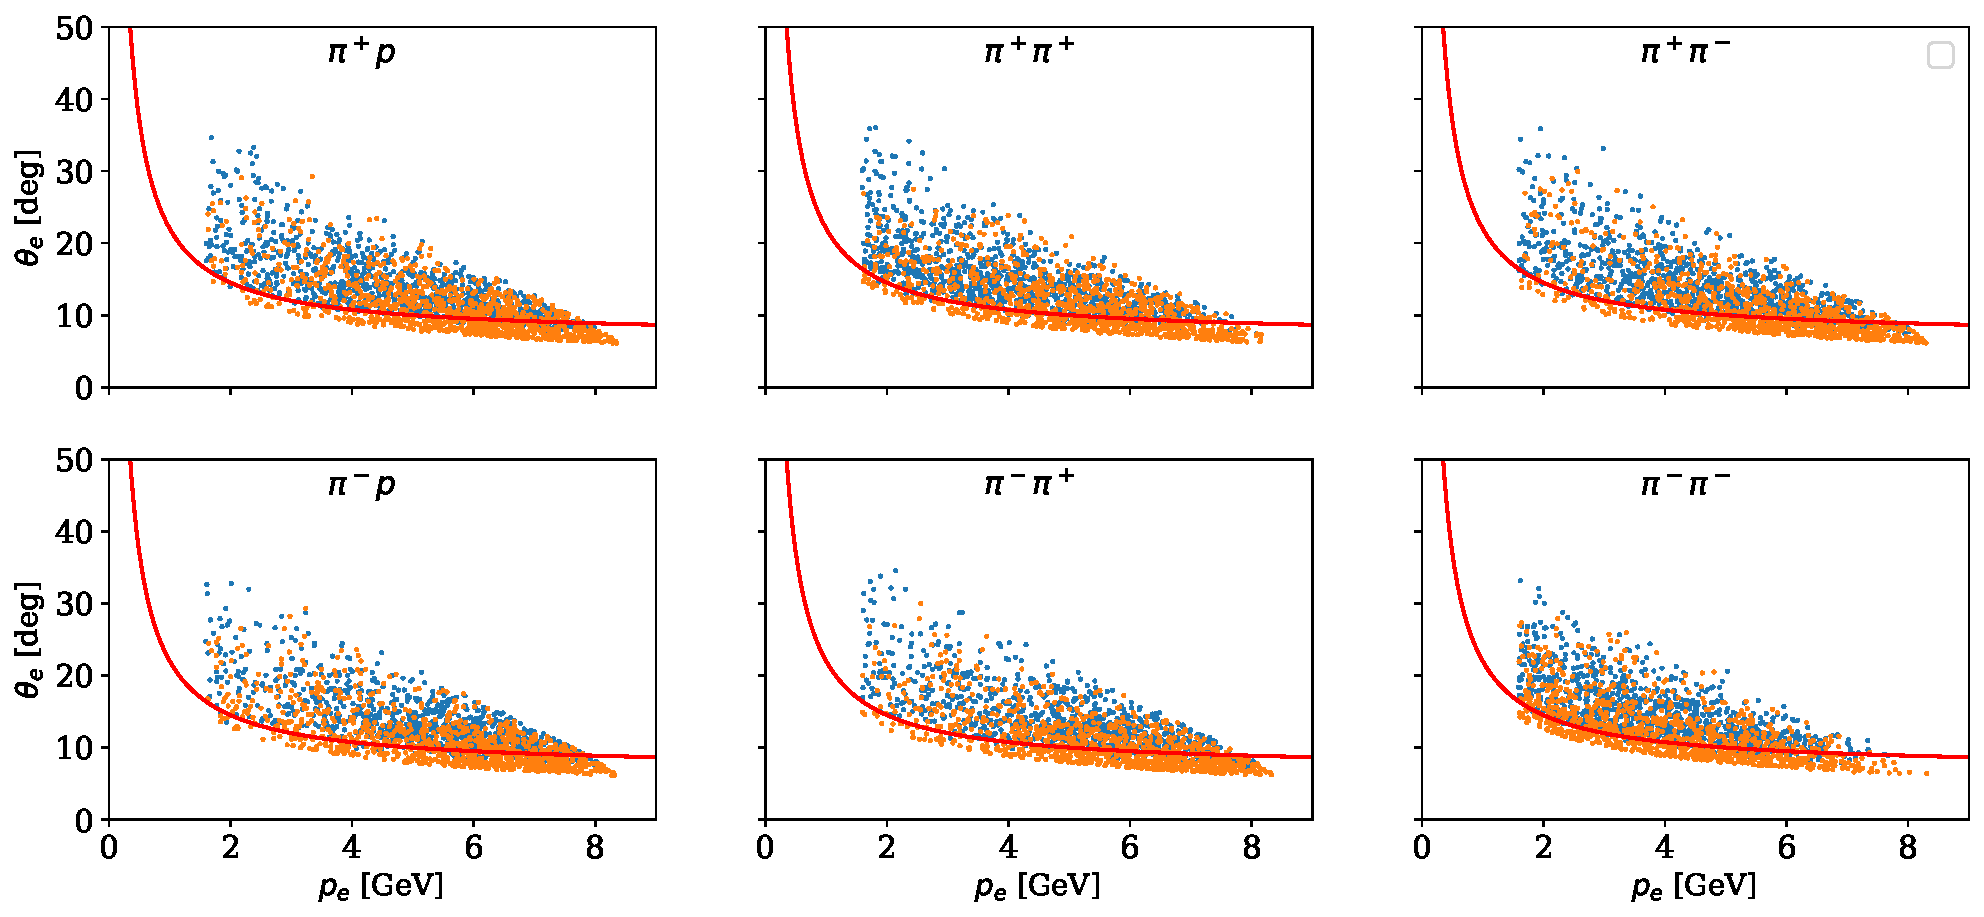
\includegraphics[width=\textwidth]{p_vs_th_inout_e}
    \caption{Electron momentum vs polar angle spectra (lab frame) for data in the in-bending (blue) and out-bending (orange) torus configurations.  The different panels represent different configurations of  di-hadron types.}
    \label{fig:p_vs_th_inout_e}
\end{figure}

\begin{figure}
    \centering
    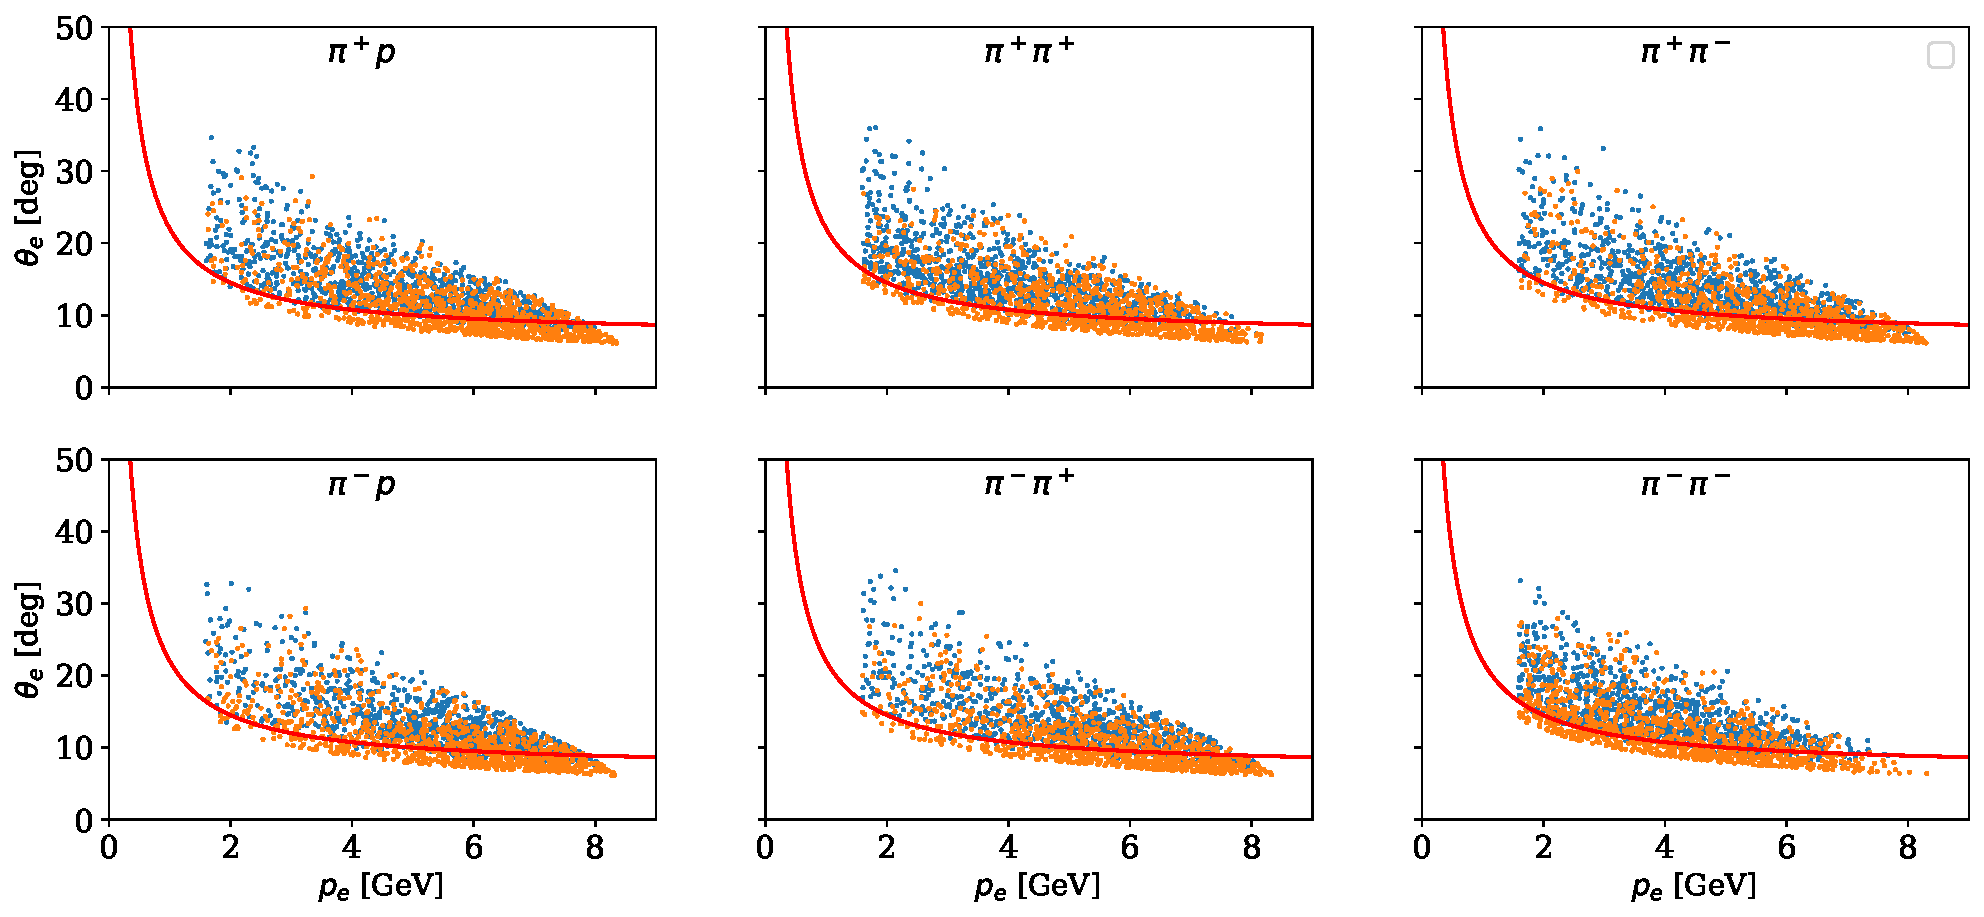
\includegraphics[width=\textwidth]{p_vs_th_inout_e}
    \caption{Same as \ref{fig:p_vs_th_inout_e} for the leading hadron's momentum and polar angle}
    \label{fig:p_vs_th_inout_h1}
\end{figure}

\begin{figure}
    \centering
    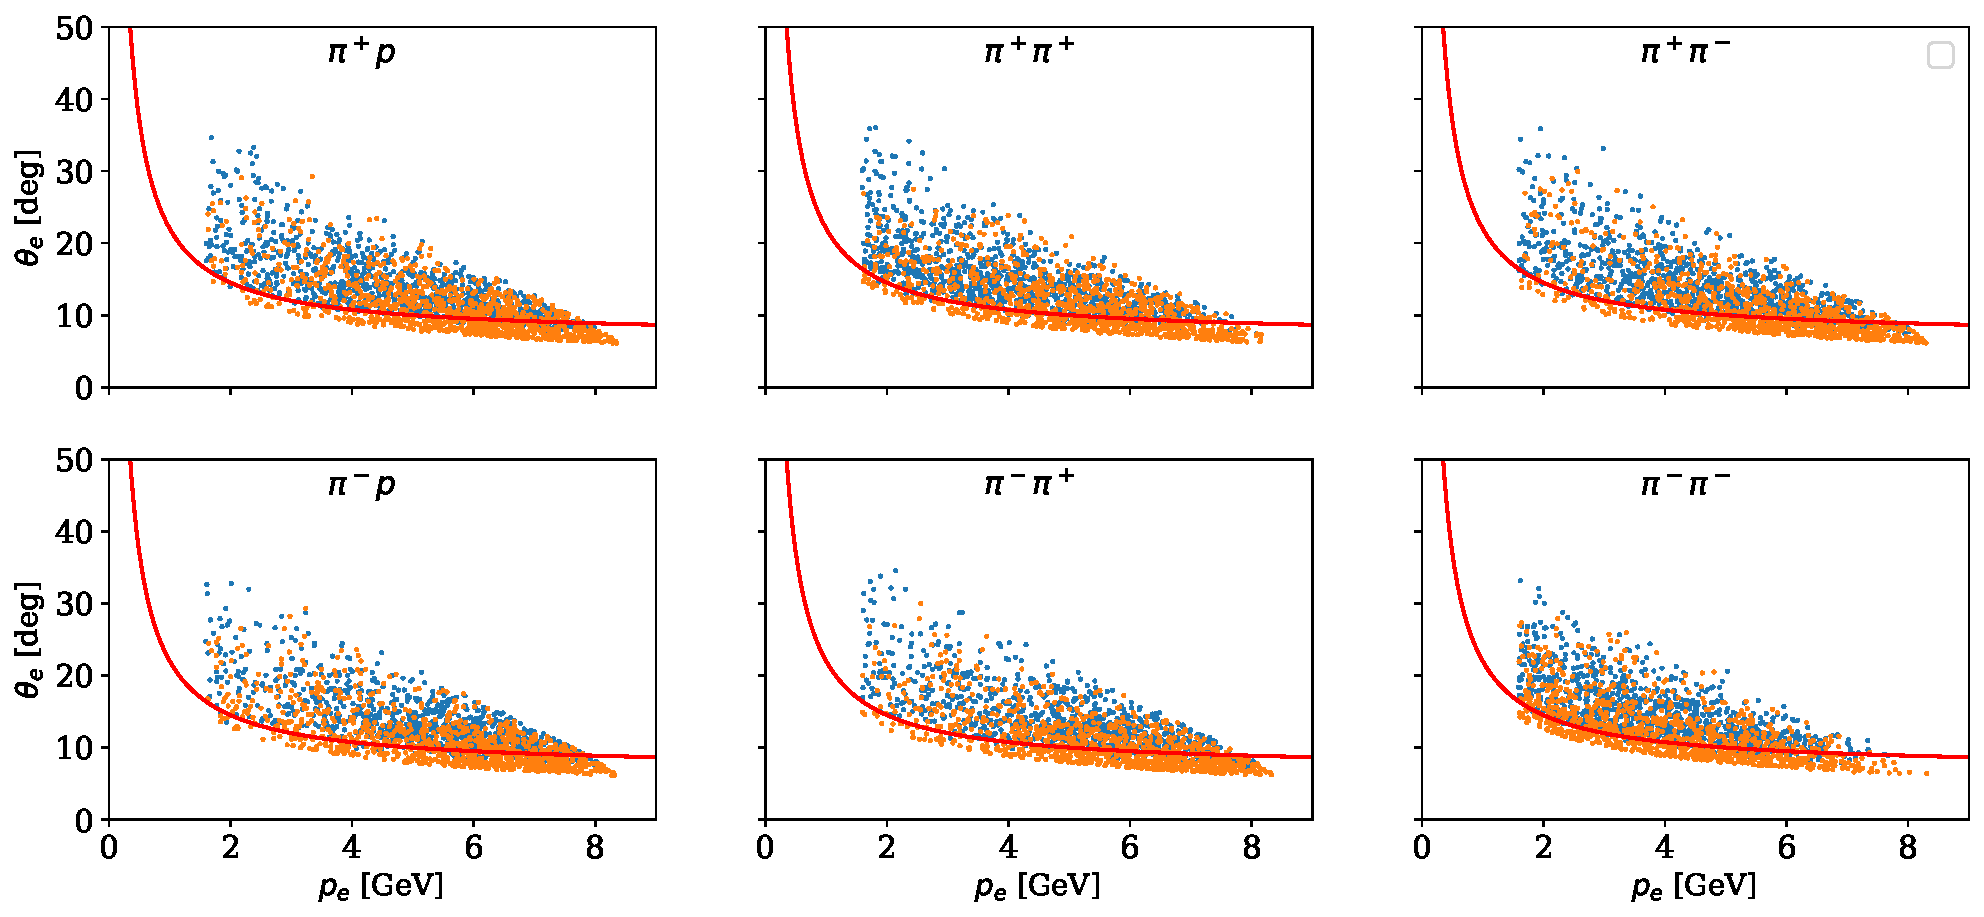
\includegraphics[width=\textwidth]{p_vs_th_inout_e}
    \caption{Same as \ref{fig:p_vs_th_inout_e} for the sub-leading hadron's momentum and polar angle}
    \label{fig:p_vs_th_inout_h2}
\end{figure}

In order to only include events in the kinematic region where the data taken with the two field polarities overlap, we used following kinematic cuts on each of the three particles ($e$,$h_1$ and $h_2$):
\begin{equation}
    \theta > 7\degree + \frac{15\degree}{p/{\rm GeV}}
\end{equation}
where $p$ and $\theta$ are the lab-frame momenta and polar angles for the particle.  This is shown as a red line in Figs.~\ref{fig:p_vs_th_inout_e}-\ref{fig:p_vs_th_inout_h2}.  



Figs.~\ref{fig:smc_pi+p_inout} through~\ref{fig:smc_pi+p-_inout} shows the same-event yields, mixed-event yields and correlation functions for each combination of particle observed ($\pi^+ p$, $\pi^- p$, $\pi^+\pi^+$, $\pi^-\pi^+$, and $\pi^+\pi^-$), with the exception of $\pi^-\pi^-$, for which we have very limited statistics. The top (bottom) panel of each figure shows the 2d functions for in-bending (out-bending) data.  The bottom panels show the 1d projections in the $\Delta y=1.5$ to 2.5 range, with inbending (outbending) data in blue (orange).  